\documentclass[11pt]{article}
\usepackage{amsmath,amssymb,amsthm}
\usepackage{tikz}
\usepackage{hyperref}
\usepackage[margin=1in]{geometry}

\newcommand{\N}{\mathbb{N}}
\newcommand{\Z}{\mathbb{Z}}
\newcommand{\Q}{\mathbb{Q}}
\newcommand{\GK}{\operatorname{GK}}
\newcommand{\CPP}{\operatorname{CPP}}
\newcommand{\IP}{\operatorname{IP}}
\newcommand{\ALCD}{\operatorname{ALCD}}
\newcommand{\qpoch}[2]{(#1;#2)_\infty}
\newcommand{\qpochn}[3]{(#1;#2)_{#3}}
\newcommand{\qbin}[2]{\genfrac{[}{]}{0pt}{}{#1}{#2}}
\DeclareMathOperator{\wt}{wt}

\theoremstyle{plain}
\newtheorem{theorem}{Theorem}
\newtheorem{conjecture}[theorem]{Conjecture}
\newtheorem{proposition}[theorem]{Proposition}
\newtheorem{lemma}[theorem]{Lemma}
\newtheorem{corollary}[theorem]{Corollary}
\theoremstyle{definition}
\newtheorem{definition}[theorem]{Definition}
\newtheorem{example}[theorem]{Example}
\newtheorem{remark}[theorem]{Remark}

\title{Peel and Glue: The Local Rule Operations\\
  on Cylindric Growth Diagrams}
\author{Robin Langer}
\date{\today}

\begin{document}
\maketitle

\begin{abstract}
We give a self-contained account of the \emph{peel} and \emph{glue}
operations on cylindric growth diagrams.  These are the inverse and
forward Burge local rules, applied one full ring at a time around the
cylinder.  They provide the mechanism for the sign-reversing involution
on the ground set $\widetilde{\mathcal{G}}_{n,c}$ of triples
$(S, U, \nu)$, where~$S$ records crossing levels, $U$ records Euler
marks, and~$\nu$ is a cylindric plane partition.
\end{abstract}

\tableofcontents


%% ============================================================
\section{The growth diagram as an onion}
\label{sec:onion}
%% ============================================================

A cylindric plane partition~$\nu$ with max entry~$n$ lives on the
outer boundary of a cylindric growth diagram.  The growth diagram has
$n$ concentric \emph{rings}, with a base partition~$\gamma$ at the
centre.

\begin{center}
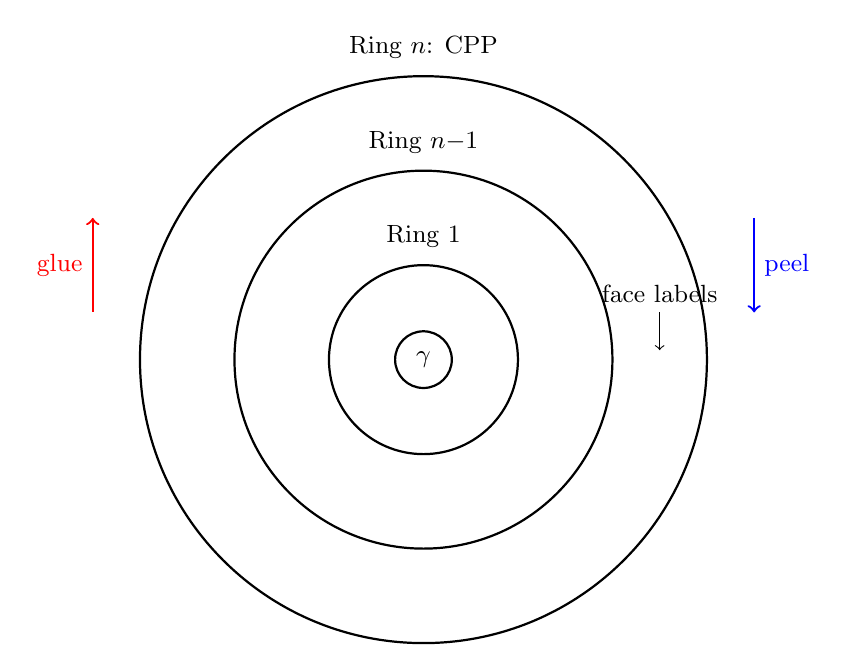
\begin{tikzpicture}[scale=1.2]
  % Rings
  \foreach \r/\lab in {3/n, 2/{n{-}1}, 1/1, 0.3/0} {
    \draw[thick] (0,0) circle (\r);
  }
  % Labels
  \node at (0, 3.3) {\small Ring $n$: CPP};
  \node at (0, 2.3) {\small Ring $n{-}1$};
  \node at (0, 1.3) {\small Ring $1$};
  \node at (0, 0)   {\small $\gamma$};
  % Face labels
  \node at (2.5, 0.7) {\small face labels};
  \draw[->,thin] (2.5, 0.5) -- (2.5, 0.1);
  % Arrows
  \draw[->,thick,blue] (3.5, 1.5) -- (3.5, 0.5)
    node[midway,right]{\small peel};
  \draw[<-,thick,red] (-3.5, 1.5) -- (-3.5, 0.5)
    node[midway,left]{\small glue};
\end{tikzpicture}
\end{center}

At each ring, the growth diagram carries two types of data:
\begin{itemize}
  \item \textbf{Vertex labels}: partitions at each vertex around the
    ring.  The outermost ring gives the CPP
    $\nu = (\mu^0, \mu^1, \ldots, \mu^{T-1})$.  The innermost vertex
    labels are all equal to the base partition~$\gamma$.
  \item \textbf{Face labels}: a non-negative integer $m(f) \geq 0$ at
    each face between two consecutive rings.  These form the ALCD
    (arbitrarily labelled cylindric diagram).
\end{itemize}

The two operations---\textbf{peel} (move inward) and \textbf{glue}
(move outward)---transfer data between the vertex labels and the face
labels, one ring at a time.


%% ============================================================
\section{The Burge local rule}
\label{sec:burge}
%% ============================================================

The local rule operates on a single \emph{face} of the growth diagram:
a diamond with four vertices.

\begin{center}
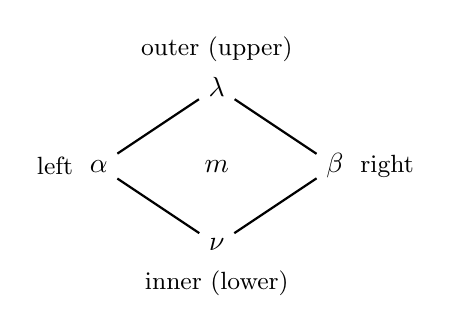
\begin{tikzpicture}[scale=1.0]
  \node (nu)     at (0, 0)  {$\nu$};
  \node (alpha)  at (-1.5, 1) {$\alpha$};
  \node (beta)   at (1.5, 1)  {$\beta$};
  \node (lambda) at (0, 2)  {$\lambda$};
  \node (m)      at (0, 1)  {$m$};
  \draw[thick] (nu) -- (alpha) -- (lambda) -- (beta) -- (nu);
  % Labels
  \node[below] at (0, -0.2) {\small inner (lower)};
  \node[above] at (0, 2.2) {\small outer (upper)};
  \node[left] at (-1.7, 1) {\small left};
  \node[right] at (1.7, 1) {\small right};
\end{tikzpicture}
\end{center}

The four vertex labels are partitions satisfying:
$\alpha/\nu$ and $\beta/\nu$ are horizontal strips (going outward),
and $\lambda/\alpha$ and $\lambda/\beta$ are horizontal strips (going
outward).  The face label~$m \geq 0$ mediates between the inner and
outer vertices.

\begin{remark}[The commutation relation]
\label{rmk:commutation}
The local rule is the bijective counterpart of the commutation
relation between vertex operators:
\[
  T(v)\, P(w) = \frac{1}{1 - vw}\, P(w)\, T(v),
\]
where $T$~is the transfer (creation) operator and $P$~is the
projection (annihilation) operator on the space of partitions.
Each application of the local rule at one face corresponds to
one commutation step: swapping a~$T$ past a~$P$.
The scalar $1/(1-vw) = \sum_{m \geq 0}(vw)^m$ generates the face
labels---the face label~$m$ records which term in the expansion
we are in.  The forward rule (glue) corresponds to the left-hand
side $T\,P$; the inverse rule (peel) corresponds to the
right-hand side $P\,T$.
\end{remark}


\subsection{The forward rule (glue direction)}
\label{sec:forward}

\begin{definition}[Burge forward rule]
\label{def:forward}
Given inner vertex~$\nu$, side vertices $\alpha, \beta$ (with
$\alpha/\nu$ and $\beta/\nu$ horizontal strips), and face
label~$m \geq 0$, the outer vertex
$\lambda = \mathfrak{U}_{\alpha,\beta}(m, \nu)$ is constructed as
follows.
\begin{enumerate}
  \item Work in \textbf{conjugate coordinates}: let $\alpha', \beta',
    \nu'$ be the conjugate partitions.
  \item Compute the \textbf{column sets}:
    \begin{align*}
      A &:= \{i \geq 1 : \alpha'_i > \nu'_i\}
        & &\text{(columns where $\alpha$ exceeds $\nu$)}, \\
      B &:= \{i \geq 1 : \beta'_i > \nu'_i\}
        & &\text{(columns where $\beta$ exceeds $\nu$)}.
    \end{align*}
    Since $\alpha/\nu$ and $\beta/\nu$ are horizontal strips,
    $\alpha'_i - \nu'_i \in \{0,1\}$ for all~$i$, so
    $A$ and $B$ are finite sets of positive integers.
  \item \textbf{Cascade}: for each $i \in A \cap B$ (in increasing
    order), let $\varepsilon(i)$ be the smallest integer $> i$ not in
    $A \cup B$ and not previously assigned.  Set
    $C := \{\varepsilon(i) : i \in A \cap B\}$.
  \item \textbf{Free columns}: let $D$ be the first $m$ elements of
    $\Z_{>0} \setminus (A \cup B \cup C)$, in increasing order.
  \item \textbf{Build $\lambda$}: set
    \[
      \lambda'_i = \nu'_i + [i \in A \cup B \cup C \cup D].
    \]
\end{enumerate}
\end{definition}

The cascade step is the heart of the local rule.  When columns~$i$
belongs to both $A$ and $B$ (i.e., both $\alpha$ and $\beta$ exceed
$\nu$ in that column), the column cannot simply be ``used twice.''
Instead, it \emph{cascades}: the overlap at column~$i$ pushes the
activation to the next available column~$\varepsilon(i) > i$.

\begin{proposition}[Weight identity]
\label{prop:weight}
\begin{equation}\label{eq:weight}
  |\lambda| = |\alpha| + |\beta| - |\nu| + m.
\end{equation}
The face label~$m$ records the \emph{excess weight}: the amount by
which $\lambda$ exceeds what $\alpha$ and $\beta$ alone would
determine.
\end{proposition}

\begin{proof}
We have $|A \cup B \cup C \cup D| = |A| + |B| - |A \cap B| + |C| + m
= |A| + |B| + m$ (since $|C| = |A \cap B|$).  And
$|\lambda| - |\nu| = |A \cup B \cup C \cup D|$,
$|\alpha| - |\nu| = |A|$, $|\beta| - |\nu| = |B|$.
\end{proof}


\subsection{The inverse rule (peel direction)}
\label{sec:inverse}

\begin{definition}[Burge inverse rule]
\label{def:inverse}
Given side vertices $\alpha, \beta$ and outer vertex~$\lambda$ (with
$\lambda/\alpha$ and $\lambda/\beta$ horizontal strips), the inverse
rule recovers $(m, \nu) = \mathfrak{U}^{-1}_{\alpha,\beta}(\lambda)$:
\begin{enumerate}
  \item Work in conjugate coordinates.
  \item Compute the \textbf{excess column sets}:
    \begin{align*}
      \bar{A} &:= \{i \geq 1 : \lambda'_i > \alpha'_i\}, \\
      \bar{B} &:= \{i \geq 1 : \lambda'_i > \beta'_i\}.
    \end{align*}
  \item \textbf{Reverse cascade}: for each $i \in \bar{A} \cap \bar{B}$
    (in \emph{decreasing} order), let $\delta(i)$ be the largest
    integer $< i$ not in $\bar{A} \cup \bar{B}$ and not previously
    assigned.
  \item \textbf{Face label}: $m := \#\{i \in \bar{A} \cap \bar{B}
    : \delta(i) \leq 0\}$ (cascade chains that ``fall off the
    edge'').
  \item \textbf{Build $\nu$}: set
    \[
      \nu'_i = \lambda'_i
        - [i \in \bar{A} \cup \bar{B} \cup \bar{C}],
    \]
    where $\bar{C} = \{\delta(i) : \delta(i) > 0\}$.
\end{enumerate}
\end{definition}

The reverse cascade ``unwinds'' the forward cascade: each overlap
column~$i \in \bar{A} \cap \bar{B}$ traces back to a smaller
column~$\delta(i) < i$.  If the trace reaches column~$0$ or below,
it contributes to the face label~$m$ instead.

\begin{proposition}
\label{prop:inverse}
The forward and inverse rules are mutual inverses:
$\mathfrak{U}^{-1}_{\alpha,\beta}
 (\mathfrak{U}_{\alpha,\beta}(m,\nu)) = (m, \nu)$.
\end{proposition}


\subsection{The cascade parameter in NILP terms}
\label{sec:cascade-nilp}

In the non-intersecting lattice path (NILP) model, the column sets
$A$ and $B$ correspond to up-steps on two adjacent paths:
\begin{itemize}
  \item $A$: columns where the left path~$p^{\alpha}$ takes an
    up-step beyond the inner path~$p^{\nu}$.
  \item $B$: columns where the right path~$p^{\beta}$ takes an
    up-step beyond~$p^{\nu}$.
\end{itemize}

The cascade columns $A \cap B$ are where \emph{both} adjacent paths
rise simultaneously---a ``pinch point'' where the gap between paths
narrows.  The cascade resolution spreads these pinch points to
neighbouring columns, preventing the paths from crossing.

The face label~$m$ counts the number of cascade chains that propagate
all the way to column~$0$.  In NILP terms, these are
\emph{cubes}---unit cells between the paths that contribute to the
total weight.

\begin{equation}\label{eq:face-cubes}
  \boxed{\;
  \text{face label } m
  = \text{number of cubes at this face}
  = \text{cascade chains reaching column } 0.
  \;}
\end{equation}


%% ============================================================
\section{Peeling a full ring}
\label{sec:full-peel}
%% ============================================================

The growth diagram for a CPP of profile~$c$ with period $T = d$ has
$T$ faces per ring.  Crucially, these $T$~faces form a \emph{closed
circle}: face~$T-1$ connects back to face~$0$, reflecting the
cylindric boundary conditions.  Peeling a full ring means
simultaneously applying the inverse local rule at all $T$~faces
around this circle, moving from ring~$k$ to ring~$k-1$.

In terms of the commutation relation
(Remark~\ref{rmk:commutation}), a full-ring peel commutes one
transfer operator past a full cycle of $T$~projection operators
around the cylinder.  Each face contributes one commutation step
and one face label; the complete circle of $T$~commutations
produces the face-label sequence $(m_0, \ldots, m_{T-1})$.

\subsection{The peel operation}

\begin{definition}[Full-ring peel]
\label{def:peel}
Let $\nu = (\mu^0, \mu^1, \ldots, \mu^{T-1})$ be a CPP with max
entry~$n$.  The \textbf{peel} at ring~$n$ produces:
\begin{enumerate}
  \item A sequence of face labels
    $(m_0, m_1, \ldots, m_{T-1})$ at ring~$n$.
  \item A smaller CPP $\nu' = (\mu'^0, \mu'^1, \ldots, \mu'^{T-1})$
    with max entry~$\leq n-1$.
\end{enumerate}
The peel is computed by applying the inverse Burge rule at each face
$f_0, f_1, \ldots, f_{T-1}$ around the ring, using the profile~$\pi$
to determine which vertex is $\alpha$ and which is $\beta$ at each
face.
\end{definition}

\begin{proposition}[Peel weight transfer]
\label{prop:peel-weight}
The total weight transferred from the CPP to the face labels is:
\begin{equation}\label{eq:peel-weight}
  |\nu| - |\nu'| = \sum_{k=0}^{T-1} m_k.
\end{equation}
Each face label~$m_k$ records the number of cubes at face~$k$ of
ring~$n$.
\end{proposition}

\begin{remark}[Iterating the peel]
Applying the peel $n$ times (once per ring, from ring~$n$ down to
ring~$1$) completely decomposes the CPP into:
\begin{itemize}
  \item The base partition $\gamma$ (the core).
  \item The face labels at all $n$ rings: an ALCD
    $\mathfrak{d} = (m_k^{(j)})$ with $j = 1, \ldots, n$ and
    $k = 0, \ldots, T-1$.
\end{itemize}
This is the growth diagram bijection
$\psi\colon (\gamma, \mathfrak{d}) \leftrightarrow \nu$
of~\cite{UNDERLYING_SET}.
\end{remark}


\subsection{The glue operation}

\begin{definition}[Full-ring glue]
\label{def:glue}
Given a CPP~$\nu'$ with max entry~$\leq n-1$ and a sequence of face
labels $(m_0, \ldots, m_{T-1})$ with $m_k \geq 0$, the \textbf{glue}
at ring~$n$ produces a CPP~$\nu$ with max entry~$\leq n$, by applying
the forward Burge rule at each face around the ring.
\end{definition}

Glue is the exact inverse of peel: peeling ring~$n$ and then gluing
it back (with the same face labels) returns the original CPP.


\subsection{What peel and glue look like}

\begin{example}[Rank~$3$, $c = (2,2,0)$, $d = 4$]
\label{ex:peel-d4}
Consider the CPP $\nu = ((1,1), (1,1,1), (1))$ with max entry~$1$
and weight~$6$.  The profile gives a cylinder of period $T = 4$.

Peeling ring~$1$ applies the inverse rule at each of the $4$~faces.
The result is:
\begin{itemize}
  \item Face labels: $(m_0, m_1, m_2, m_3)$ --- recording the cubes
    at each face of ring~$1$.
  \item Inner CPP: the base partition~$\gamma$ (since max entry
    was~$1$, one peel reaches the core).
\end{itemize}
The total face-label weight $\sum m_k = |\nu| - |\gamma|$.
\end{example}


%% ============================================================
\section{The ground set and the involution}
\label{sec:ground-set}
%% ============================================================

\subsection{The three-component ground set}

We begin from two definitions.  The generating function for
cylindric plane partitions with profile~$c$ is
\begin{equation}\label{eq:GK}
  \GK_c(z,q) = \sum_{\pi \in \CPP(c)}
    z^{\max(\pi)}\, q^{|\pi|},
\end{equation}
where $\max(\pi)$ is the largest entry and $|\pi|$ is the
sum of all entries.  The \emph{$Q$-polynomial} is
\begin{equation}\label{eq:Q-def}
  Q_{n,c}(q)
  = \qpochn{q}{q}{n}
    \cdot [z^n]\bigl(\qpoch{zq}{q} \cdot \GK_c(z,q)\bigr).
\end{equation}

\noindent
We now expand~\eqref{eq:Q-def} to derive the ground set.
Write $g_m(q) = [z^m]\,\GK_c(z,q)$, so that
$\GK_c = \sum_m g_m\, z^m$.  The Euler product
$\qpoch{zq}{q} = \prod_{k \geq 1}(1 - zq^k)$ expands as
\[
  \qpoch{zq}{q} = \sum_{J} (-1)^{|J|}\, z^{|J|}\,
    q^{\sigma(J)},
\]
where $J$ ranges over all finite subsets of
$\{1, 2, 3, \ldots\}$ and $\sigma(J) = \sum_{k \in J} k$.
Multiplying by $\GK_c$ and extracting $[z^n]$ (which forces
$|J| + m = n$, so $m = n - |J|$ and $|J| \leq n$):
\[
  f_n(q) := [z^n]\bigl(\qpoch{zq}{q} \cdot \GK_c\bigr)
  = \sum_{j=0}^{n} (-1)^j
    \left(\sum_{\substack{J \subseteq \{1,2,\ldots\}
    \\[2pt] |J| = j}} q^{\sigma(J)}\right)
    g_{n-j}.
\]
The sum over $j$-element subsets of $\{1,2,\ldots\}$
equals $q^{j(j+1)/2}/(q)_j$ (the minimal such subset
$\{1, \ldots, j\}$ has sum $j(j+1)/2$; the excess is an
unrestricted partition into at most $j$ parts).  So
$f_n = \sum_{j} (-1)^j\, q^{j(j+1)/2}\, g_{n-j} / (q)_j$.

Multiplying by $(q)_n$ and splitting $(q)_n/(q)_j
= \qbin{n}{j} \cdot (q)_{n-j}$:
\[
  Q_n = \sum_{j=0}^{n} (-1)^j\, q^{j(j+1)/2}\,
    \qbin{n}{j}\, (q)_{n-j}\, g_{n-j}.
\]
Now use the identity $q^{j(j+1)/2}\,\qbin{n}{j}
= \sum_{\substack{S \subseteq \{1,\ldots,n\} \\
|S|=j}} q^{\sigma(S)}$ (the minimal $j$-element subset of
$\{1, \ldots, n\}$ is $\{1, \ldots, j\}$; the $q$-binomial
counts the excess), and expand
$(q)_m = \prod_{k=1}^{m}(1-q^k)
= \sum_{U \subseteq \{1,\ldots,m\}} (-1)^{|U|}\,q^{\sigma(U)}$.
Setting $m = n - j$:
\begin{equation}\label{eq:Q-triple}
  \boxed{\;
  Q_{n,c}(q)
  = \sum_{(S, U, \nu) \in \widetilde{\mathcal{G}}_{n,c}}
    (-1)^{|S| + |U|}\,
    q^{\sigma(S) + \sigma(U) + |\nu|},
  \;}
\end{equation}
where the \textbf{ground set} is
\begin{equation}\label{eq:ground-set}
  \widetilde{\mathcal{G}}_{n,c}
  = \bigsqcup_{j=0}^{n}
  \left\{(S, U, \nu) :
    \begin{array}{l}
      S \subseteq \{1, \ldots, n\},\; |S| = j, \\[2pt]
      U \subseteq \{1, \ldots, n-j\}, \\[2pt]
      \nu \in \CPP(c),\; \max(\nu) = n - j
    \end{array}
  \right\}.
\end{equation}

Each component of the triple arises from a different factor
in~\eqref{eq:Q-def}:
\begin{center}
\renewcommand{\arraystretch}{1.3}
\begin{tabular}{l|l|l|l}
\textbf{Component} & \textbf{Source} & \textbf{Sign} & \textbf{Weight}
\\ \hline
$S \subseteq \{1,\ldots,n\}$
  & $q^{j(j+1)/2}\qbin{n}{j}$ from $(q)_n/\!(q)_j$
  & $(-1)^{|S|}$
  & $\sigma(S) = \sum_{s \in S} s$
\\
$U \subseteq \{1,\ldots,m\}$
  & $(q)_m$ factor
  & $(-1)^{|U|}$
  & $\sigma(U) = \sum_{u \in U} u$
\\
$\nu \in \CPP(c)$, $\max = m$
  & $g_m = [z^m]\,\GK_c$
  & $+1$
  & $|\nu|$
\end{tabular}
\end{center}

\noindent
Here $m = n - |S|$ is the max entry of the CPP\@.
The larger the crossing set~$S$, the fewer rings the CPP
has: a triple with $|S| = j$ uses a CPP with only $n - j$
rings in the growth diagram.  At one extreme ($S = \emptyset$),
the CPP occupies all $n$~rings; at the other ($|S| = n$),
the CPP is empty and all weight is carried by~$S$.
The sign is $(-1)^{|S| + |U|}$ and the weight is
$\sigma(S) + \sigma(U) + |\nu|$.  All three components are
manifestly non-negative objects (subsets and CPPs); the signs
come \emph{only} from the exponent $(-1)^{|S|+|U|}$.

\begin{remark}[$S$ as crossing levels]
\label{rmk:S-levels}
The triple $(S, U, \nu)$ allocates $n$~potential levels into two
roles: the $m = n - |S|$ levels \emph{not} in~$S$ are occupied by
the CPP (one ring per level), while the $|S|$ levels in~$S$ are
spent as \emph{crossings}.  Each element $k \in S$ is the index of
a level allocated to crossings rather than to the CPP, contributing
weight~$q^k$ and sign~$-1$.

One might hope that $k$ equals the number of boxes at the
corresponding ring (the face-label total at that level).  But this
cannot work in general: two different rings could have the same
box count, violating the requirement that $S$ is a \emph{set} of
distinct elements.  The box count could also be~$0$ or exceed~$n$.
So the elements of~$S$ are abstract level indices from the
$q$-binomial expansion, not face-label totals.

In the involution, when we peel a ring and add an element to~$S$,
we must choose $k \in \{1, \ldots, n\} \setminus S$ and adjust~$U$
so that weight conservation holds.  The face-label total at the
peeled ring constrains this choice but does not determine it
uniquely---this is part of the canonical choice
(Section~\ref{sec:canonical}).
\end{remark}

\begin{remark}[$U$ as compressed rings]
\label{rmk:U-compressed}
The subset $U \subseteq \{1, \ldots, m\}$ plays an analogous but
subtler role to~$S$.  It comes from expanding the factor
$(q)_m = \prod_{k=1}^{m}(1-q^k)$: at each ring~$k$, we choose
either the $1$~term (ring~$k$ is uncompressed) or the $-q^k$~term
(ring~$k$ is compressed, contributing weight~$k$ and sign~$-1$).

The element $i \in U$ means: \emph{ring~$i$ has been compressed}.
The ring is still present in the CPP---unlike~$S$, where the ring
is destroyed entirely---but $i$~units of its face-label weight
have been extracted and stored in~$U$.  The ring is lighter than
it would otherwise be.

In this picture, a triple $(S, U, \nu)$ represents a single CPP
that has been compressed in \textbf{two stages}:
\begin{enumerate}
  \item \textbf{Structural compression} ($\to S$):\;
    interior-crush (Section~\ref{sec:crushing}) the levels in~$S$
    out of the NILP tower.  Each $k \in S$ removes level~$k$,
    collapsing two adjacent levels into one.  The CPP goes from
    max entry~$n$ to max entry~$m = n - |S|$.
  \item \textbf{Weight compression} ($\to U$):\;
    at each remaining ring~$i \in U$, peel out $i$~units of
    face-label weight.  The ring stays but gets lighter.
\end{enumerate}
What remains after both stages is~$\nu$.  To \textbf{reconstruct}
the full CPP, reverse the process: first un-peel the rings of~$U$
(inject weight back), then un-crush the levels of~$S$ (glue the
removed levels back in).

The sign $(-1)^{|S|+|U|}$ counts the total number of
compressions: $|S|$~structural crushes plus $|U|$~weight
extractions.  The involution toggles one compression---either
crushing or uncrushing one more level (changing~$|S|$), or
peeling or unpeeling one more ring (changing~$|U|$)---thereby
changing $|S|+|U|$ by~$\pm 1$.
\end{remark}

\begin{remark}[Multiple compressions of a single CPP]
\label{rmk:multiple-compressions}
A single CPP~$\tilde{\nu}$ with max entry~$n$ can be compressed
into many different triples, depending on which levels are crushed
(choice of~$S$) and which rings have weight extracted
(choice of~$U$).  For instance, with max entry~$3$, some of the
triples representing different compressions of~$\tilde{\nu}$:
\begin{center}
\renewcommand{\arraystretch}{1.3}
\begin{tabular}{l|l|c}
\textbf{Triple} & \textbf{Compressions} & \textbf{Sign}
\\ \hline
$(\emptyset,\; \emptyset,\; \tilde{\nu})$
  & none & $+1$ \\
$(\{3\},\; \emptyset,\; \nu')$
  & crush level $3$ & $-1$ \\
$(\{2\},\; \emptyset,\; \nu'')$
  & crush level $2$ & $-1$ \\
$(\emptyset,\; \{1\},\; \nu''')$
  & peel ring $1$ & $-1$ \\
$(\{2,3\},\; \emptyset,\; \nu^{(4)})$
  & crush levels $2$ and $3$ & $+1$ \\
$(\{3\},\; \{1\},\; \nu^{(5)})$
  & crush level $3$, peel ring $1$ & $+1$
\end{tabular}
\end{center}
These are all distinct elements of the ground set, with different
signs and generally different total weights.  The ground set
$\widetilde{\mathcal{G}}_{n,c}$ is the space of \emph{all possible
compressions} of all CPPs with max entry up to~$n$.

The conjecture $Q_n \in \N[q]$ therefore says: for every CPP and
every odd-depth compression of it (with $|S| + |U|$ odd), there
exists a matching even-depth compression at the same total weight.
The involution's job is to find these matchings systematically.
\end{remark}

\begin{remark}[$S$, $U$, and the ALCD]
\label{rmk:S-U-ALCD}
The partial disassembly picture should not be confused with the
ALCD\@.  The \textbf{ALCD} $\mathfrak{d} = (m_k^{(j)})$ is the
growth diagram's native representation: $T$~face labels at each of
$n$~rings, equivalent to the CPP via the growth diagram bijection
(Section~\ref{sec:full-peel}).  It carries \emph{no sign} and
records the complete internal structure.

The components $S$ and~$U$ are \textbf{sign-carrying} objects from
the algebraic expansion of the Euler products
in~\eqref{eq:Q-def}: $S$ carries sign~$(-1)^{|S|}$, $U$~carries
sign~$(-1)^{|U|}$, and the CPP~$\nu$ carries sign~$+1$.  When the
involution removes a ring (into~$S$), the ALCD loses a full row of
$T$~face labels and $S$~gains one number.  When the involution
extracts weight (into~$U$), the ALCD's face labels at ring~$i$
are reduced and $U$~gains one number.  In both cases, detailed
structure is compressed into a single scalar.
\end{remark}


\subsection{Compression of a CPP}
\label{sec:compression}

The ground set has a natural interpretation: each triple
$(S, U, \nu)$ represents a \textbf{compression} of a cylindric
plane partition.  A compression selects certain rings to crush
or mark, producing a smaller, lighter object that still records
all the weight.

\begin{definition}[Compression]
\label{def:compression}
Let $\tilde{\nu}$ be a CPP with max entry~$n$.  A
\textbf{compression} of~$\tilde{\nu}$ is a triple
$(S, U, \nu)$ obtained in two stages:
\begin{enumerate}
  \item \textbf{Structural compression} (choosing~$S$): select a
    subset $S \subseteq \{1, \ldots, n\}$ of levels to crush.
    Crushing level~$k$ applies the inverse Burge rule at all
    $T$~faces of ring~$k$, merging levels $k{-}1$ and~$k$.  After
    crushing all levels in~$S$, the residual CPP has max
    entry~$m = n - |S|$.  Each crushed level contributes sign~$-1$
    and weight~$k$ (the level index).
  \item \textbf{Weight compression} (choosing~$U$): select a
    subset $U \subseteq \{1, \ldots, m\}$ of remaining rings to
    mark.  Marking ring~$i$ extracts $i$~units of face-label
    weight from the growth diagram at ring~$i$, storing them as
    the Euler mark~$i \in U$.  The CPP~$\nu$ is the residual
    after both stages.  Each mark contributes sign~$-1$ and
    weight~$i$.
\end{enumerate}
The total sign is $(-1)^{|S|+|U|}$ and the total weight is
$\sigma(S) + \sigma(U) + |\nu|$.
\end{definition}

\noindent
At one extreme ($S = U = \emptyset$), no compression occurs and
the triple is simply $(\emptyset, \emptyset, \tilde{\nu})$ with
sign~$+1$.  At the other extreme ($|S| = n$), every level is
crushed, the CPP is empty, and all weight is carried by~$\sigma(S)$.

\begin{remark}[The ground set as a space of compressions]
\label{rmk:compression-space}
A single CPP~$\tilde{\nu}$ with max entry~$n$ generates $2^n$
compressions (one for each choice of~$S$), and each residual CPP
generates further choices of~$U$.  Different compressions of the
same CPP are distinct elements of the ground set with
(generally) different signs and total weights.

The full ground set $\widetilde{\mathcal{G}}_{n,c}$ is the union
of all compressions of all CPPs with max entry up to~$n$.
The conjecture $Q_n \in \N[q]$ asserts that across all CPPs and
all their compressions, the positive-signed terms outweigh the
negative-signed ones at every power of~$q$.  The involution's
task is to pair each negative compression with a positive one at
the same total weight.
\end{remark}


\subsection{Two levels of compression}

The ground set~\eqref{eq:ground-set} can be compressed by absorbing
the internal signs.

\paragraph{Level~2 (pairs).}
If $h_{m,c}(q) := \qpochn{q}{q}{m} \cdot f_{m,c}(q) \in \N[q]$
(i.e., all coefficients are non-negative), then the $(U, \nu)$ data
can be compressed into a single object~$\tau$ counted by~$h_{m,c}(q)$:
\begin{equation}\label{eq:level2}
  \mathcal{G}_{n,c} = \bigsqcup_{j=0}^{n}
  \{(S, \tau) : S \subseteq \{1,\ldots,n\},\; |S| = j,\;
  \tau \in \mathcal{H}_{n-j,c}\},
\end{equation}
with sign $(-1)^{|S|}$.  The Euler signs from~$U$ cancel internally.

This compression works when $d \not\equiv 0 \pmod{3}$ (verified for
$d = 1, 2, 4, 5, 7, 8$).  When $d \equiv 0 \pmod{3}$, the polynomial
$h_{m,c}(q)$ has negative coefficients, and the compression fails:
one must work with the full triples~\eqref{eq:ground-set}.

\paragraph{Level~3 (triples).}
This is the universal description.  Every component is manifestly
non-negative: $S$ and $U$ are subsets (counted by~$1$), and $\nu$ is
a CPP (counted by~$f_{m,c}(q) \in \N[q]$).  The signs come
\emph{only} from $(-1)^{|S|+|U|}$, never from the objects themselves.
The non-negativity of $h_m$ is irrelevant at this level.


\subsection{Peel and glue ARE the involution}
\label{sec:involution}

The central claim of this note is:

\begin{quote}
\emph{The sign-reversing involution on $\widetilde{\mathcal{G}}_{n,c}$
is not merely ``implemented by'' peel and glue.  Every non-trivial
move of the involution IS a peel or glue operation---there is no other
mechanism available.}
\end{quote}

To see why, consider what the involution must do.  Suppose a map
$\iota\colon \widetilde{\mathcal{G}}_{n,c} \to
\widetilde{\mathcal{G}}_{n,c}$ exists that proves
$Q_{n,c}(q) \in \N[q]$.  Such a map is not yet constructed---its
existence is equivalent to the conjecture---but we can deduce what
form it must take.  It acts on triples $(S, U, \nu)$ and must
satisfy three constraints:
\begin{enumerate}
  \item $\iota^2 = \operatorname{id}$ (involutive).
  \item If $\iota(S, U, \nu) = (S', U', \nu') \neq (S, U, \nu)$,
    then $|S'| + |U'| \equiv |S| + |U| + 1 \pmod{2}$
    (sign reversal).
  \item $\sigma(S) + \sigma(U) + |\nu|
    = \sigma(S') + \sigma(U') + |\nu'|$
    (weight preservation).
\end{enumerate}
If such an~$\iota$ exists, the fixed-point generating function
gives the $Q$-polynomial:
\begin{equation}\label{eq:fixed-points}
  Q_{n,c}(q) = \sum_{\substack{(S,U,\nu) \\
    \iota(S,U,\nu)=(S,U,\nu)}}
    (-1)^{|S|+|U|}\, q^{\sigma(S)+\sigma(U)+|\nu|}.
\end{equation}

\noindent
We now show that $\iota$, if it exists, must be a peel or a glue.

Sign reversal requires changing $|S| + |U|$ by~$\pm 1$.  Since
$S$~and~$U$ are subsets (discrete objects), this means either adding
or removing a single element from $S$ or~$U$.  But adding or
removing an element changes the weight, so the CPP~$\nu$ must
compensate.  The \emph{only} way to adjust a CPP's weight while
preserving its cylindric structure is to peel or glue a ring in the
growth diagram.  There is no ``move a box'' operation on CPPs that
bypasses the growth diagram: the interlacing constraints between the
three partitions $(\nu^1, \nu^2, \nu^3)$ are too rigid.

This means that $\iota$ is not something separate that ``uses''
peel and glue as subroutines.  Each application of~$\iota$ to a
non-fixed-point triple IS exactly one peel or one glue:
\[
  \iota(S, U, \nu) =
  \begin{cases}
    \text{peel: strip a ring from $\nu$, store in $S$ or $U$}
    & \text{(triple gets ``smaller''),} \\
    \text{glue: take from $S$ or $U$, build a ring on $\nu$}
    & \text{(triple gets ``bigger'').}
  \end{cases}
\]
Every non-fixed-point pair $\{x, \iota(x)\}$ consists of one
``big'' triple and one ``small'' triple.  The map~$\iota$ sends the
big one to the small one via peel, and the small one back to the big
one via glue.  Since peel and glue are mutual inverses
(Proposition~\ref{prop:inverse}), $\iota^2 = \operatorname{id}$.

The entire involution is therefore encoded in a single
\textbf{decision rule}: given a triple, does it get peeled or glued,
and at which ring?  This decision rule is the \emph{canonical
choice} of Section~\ref{sec:canonical}.  The mechanism is given;
the logic is missing.

The two fundamental moves are as follows.

\begin{definition}[The two fundamental moves]
\label{def:two-moves}
Given a triple $(S, U, \nu)$ with $m = n - |S|$, the involution
performs \emph{exactly one} of the following:

\medskip
\noindent\textbf{Move~U (Euler peel/glue): trade a mark for weight.}
Change $|U|$ by~$\pm 1$ while keeping the CPP's max entry~$m$ fixed.
\[
  (S, U, \nu) \;\longleftrightarrow\; (S,\; U \triangle \{i\},\; \nu')
  \qquad\text{where } \max(\nu') = m,\; |\nu'| = |\nu| \mp i.
\]

\noindent
\textsc{Peel direction} (add a mark):
Choose $i \in \{1, \ldots, m\} \setminus U$.  Redistribute
weight~$i$ from~$\nu$ to~$U$:  this means peeling cubes from the
interior of the growth diagram (modifying face labels at ring~$i$)
to extract exactly $i$~units of weight, then recording the mark
$i \in U$.  The CPP shrinks: $|\nu'| = |\nu| - i$.

\smallskip\noindent
\textsc{Glue direction} (remove a mark):
Choose $i \in U$.  Remove the mark and inject weight~$i$ back
into~$\nu$: this means inserting face-label weight at ring~$i$
via the forward Burge rule, growing the CPP by~$i$ units.

\medskip
\noindent\textbf{Move~S (crossing peel/glue): trade a level for
a ring.}
Change $|S|$ by~$\pm 1$, which changes the CPP's max entry.
\[
  (S, U, \nu) \;\longleftrightarrow\;
  (S \triangle \{k\},\; U',\; \nu')
  \qquad\text{where } \max(\nu') = m \mp 1.
\]

\noindent
\textsc{Peel direction} (add a crossing):
Apply the inverse Burge rule (Section~\ref{sec:inverse}) to the
\emph{outermost ring} of~$\nu$, extracting face labels
$(m_0, \ldots, m_{T-1})$.  Record the level $k = m$ in~$S$, and
adjust~$U$ to $U' \subseteq \{1, \ldots, m-1\}$.  The CPP loses
its top ring: $\max(\nu') = m - 1$.

\smallskip\noindent
\textsc{Glue direction} (remove a crossing):
Take a level~$k \in S$, construct face labels from the available
weight budget, and apply the forward Burge rule
(Section~\ref{sec:forward}) to add a new outermost ring.  The CPP
gains a top ring: $\max(\nu') = m + 1$.
\end{definition}

\begin{remark}[Why only two moves, not three]
\label{rmk:two-not-three}
One might consider a third operation---\textbf{Move~C}
(cross-to-mark conversion)---that trades an element of~$S$ for an
element of~$U$.  Since $|S|$ decreases by~$1$ and $|U|$ increases
by~$1$, the total $|S| + |U|$ is unchanged, so the sign is
preserved.  Move~C is therefore \emph{sign-neutral}: it cannot
serve as the involution step itself.  It could in principle serve
as a preparatory conjugation (apply Move~C, then Move~U, then
undo Move~C), but this composite operation reduces to a single
Move~S\@.  The two fundamental moves suffice.
\end{remark}

\begin{remark}[Properties of peel and glue]
\label{rmk:peel-glue-properties}
Both fundamental moves have three key properties.

\smallskip\noindent
\textbf{Weight-preserving.}\;
Peel does not destroy weight---it \emph{redistributes} it.  By the
weight identity (Proposition~\ref{prop:weight}), a full-ring peel
satisfies $|\nu| = |\nu'| + \sum_k m_k$: the CPP shrinks, and the
extracted face labels carry the difference.  In the involution
context, that face-label weight flows into~$\sigma(S)$ or~$\sigma(U)$,
so the total $\sigma(S) + \sigma(U) + |\nu|$ is preserved.  Glue
reverses the flow: weight moves from $S$ or~$U$ back into the CPP\@.

\smallskip\noindent
\textbf{Sign-reversing.}\;
Move~U adds or removes an element from~$U$, changing $|U|$
by~$\pm 1$.  Move~S adds or removes an element from~$S$,
changing $|S|$ by~$\pm 1$.  Either way, the sign
$(-1)^{|S|+|U|}$ flips.  This is what makes the cancellation
work: each peel--glue pair matches a positive triple with a
negative triple of the same weight.

\smallskip\noindent
\textbf{Mutually inverse (not self-inverse).}\;
Peel and glue are inverses of each other
(Proposition~\ref{prop:inverse}): peel followed by glue with the
same face labels returns the original CPP\@.  But peel is
\emph{not} an involution---applying it twice strips two rings.
The involution~$\iota$ is built from this inverse pair: it applies
peel in one direction and glue in the other, so that
$\iota^2 = \operatorname{id}$.
\end{remark}

\subsection{The canonical choice}
\label{sec:canonical}

The preceding analysis shows that the \emph{mechanism} of the
involution is completely determined: it must be a peel or a glue.
What remains open is the \textbf{canonical choice}: given a
non-fixed-point triple $(S, U, \nu)$, which specific move does the
involution apply?

The requirements on this choice are:
\begin{enumerate}
  \item \textbf{Deterministic}: the choice depends only on
    $(S, U, \nu)$, with no auxiliary data.
  \item \textbf{Self-inverse}: if the chosen move sends
    $(S, U, \nu) \mapsto (S', U', \nu')$, then the chosen move at
    $(S', U', \nu')$ must send it back to $(S, U, \nu)$.
  \item \textbf{Weight-preserving}: the move must transfer
    \emph{exactly} the right amount of weight between components.
  \item \textbf{Well-defined on fixed points}: the triples where no
    canonical peel exists are precisely the fixed points, and their
    generating function must equal~$Q_{n,c}(q)$.
\end{enumerate}

\begin{remark}[The peel/glue dichotomy]
For each non-fixed-point triple, the involution either peels (extracting
structure from $\nu$ into $S$ or~$U$) or glues (injecting structure from
$S$ or~$U$ back into~$\nu$).  The triple and its image form a
\emph{peel--glue pair}: one member is in the ``peeled'' state and the
other in the ``glued'' state.  The canonical choice amounts to a
consistent rule for deciding which state a given triple is in.

In Franklin's classical involution on Euler's pentagonal number theorem,
the analogous choice is: ``does the smallest part fit in the diagonal
slope, or does the diagonal slope fit in the bottom row?''  The
involution has a single canonical comparison.  For the cylindric case,
the analogous comparison must account for three interlacing partitions
wrapped around a cylinder---a fundamentally harder combinatorial
problem.
\end{remark}

\begin{remark}[The asymmetry of peel and glue]
\label{rmk:asymmetry}
Peel and glue are mutual inverses (Proposition~\ref{prop:inverse}),
but they are \emph{not} symmetric in terms of information.

\textbf{Peel is deterministic.}\;
Given a CPP~$\nu$, the inverse Burge rule at each face is a
well-defined function: the side vertices~$\alpha, \beta$ and outer
vertex~$\lambda$ uniquely determine the inner vertex~$\nu$ and face
label~$m$.  A full-ring peel produces a unique smaller
CPP~$\nu'$ and unique face labels $(m_0, \ldots, m_{T-1})$.
No choices are involved.

\textbf{Glue requires data.}\;
The forward Burge rule is equally deterministic, but it takes the
face labels as \emph{input}.  To glue a ring onto~$\nu'$, one must
specify $(m_0, \ldots, m_{T-1})$.  Different face labels produce
different CPPs.

This asymmetry has a direct consequence for the ground set.  The
triple $(S, U, \nu)$ does not encode enough information to
reconstruct a unique ``uncompressed'' CPP\@.  For the $S$~component:
the level index $k \in S$ records \emph{which} ring was crushed, but
not the $T$~face labels that were there---those are lost.  For
the $U$~component: the subset~$U$ and the CPP~$\nu$ are
algebraically independent objects (from different factors in the
$Q$-polynomial expansion), so there is no literal extraction to
reverse.

In the involution, this asymmetry concentrates the difficulty
in the glue direction: peeling a non-fixed-point triple is
automatic, but gluing its partner back requires choosing the
right face labels.  The canonical choice
(Section~\ref{sec:canonical}) must resolve this.
\end{remark}

\begin{remark}[Contrast with the LGV involution]
\label{rmk:lgv}
In the classical Lindstr\"om--Gessel--Viennot setting, the
sign-reversing involution on intersecting lattice path families is
purely local: find the \emph{first} intersection point of two paths,
swap their tails beyond that point, and the crossing is resolved.
The set of crossing points changes by exactly one element, the sign
flips, and the weight is automatically preserved because the same
edges are traversed (just by different paths).

One might hope that the crossing set $S \subseteq \{1, \ldots, n\}$
in our ground set plays the same role: $S$ records ``crossing
levels'' in the NILP tower, and the involution ``uncrosses'' them
one at a time.  This interpretation is morally correct---$S$ does
record which levels carry crossings---but the mechanism is
fundamentally different.

The LGV paths live in the plane, and a tail-swap is a local
operation that preserves all path constraints.  Our paths live on a
\emph{cylinder}: three paths wrap around with cyclic interlacing
$\nu^1 \unrhd \nu^2 \unrhd \nu^3 \unrhd \nu^1$.  Swapping tails
at a single level would violate these interlacing conditions at
other levels.  Instead, ``uncrossing level~$k$'' requires a
\emph{whole-ring} restructuring of the CPP via peel/glue:
the inverse Burge rule is applied at all $T$~faces around the
circle, globally adjusting the path geometry to accommodate the
change in~$S$.  The crossing set changes by one element (as in
LGV), but the cost is a full ring operation (unlike LGV).
\end{remark}

\begin{remark}[Why: the determinant is missing]
\label{rmk:determinant}
The deeper reason the LGV involution fails is that the underlying
generating function is not a determinant.

In the classical setting, the Jacobi--Trudi formula
$s_\lambda = \det(h_{\lambda_i - i + j})$
expresses the Schur function as a determinant.  The LGV lemma
interprets this: the expansion
$\det = \sum_\sigma \operatorname{sgn}(\sigma)\,\prod a_{i,\sigma(i)}$
runs over permutations~$\sigma$, each corresponding to a path
family.  The sign-reversing involution (uncross, swap tails)
exploits the determinantal structure: swapping two rows of a
determinant flips the sign, and that algebraic fact has a direct
combinatorial counterpart.

For cylindric partitions, $\GK_c(z,q)$ is a \emph{trace} of a
product of transfer matrices around the cylinder, not a
determinant.  The cylindric Schur functions do not satisfy
Jacobi--Trudi.  The alternating-sum structure of
$Q_n = \sum (-1)^{|S|+|U|}\, q^{\sigma(S)+\sigma(U)+|\nu|}$
arises instead from the Euler factors $\qpoch{zq}{q}$ and
$\qpochn{q}{q}{m}$ applied to this non-determinantal generating
function (see the derivation in Section~\ref{sec:ground-set}).

So the $Q$-polynomial has the \emph{form} of a determinant
expansion (a signed sum where massive cancellation is expected)
without the \emph{source} being a determinant.  The involution
must accomplish the same cancellation that the LGV involution
achieves for genuine determinants, but without the algebraic
shortcut that determinantal structure provides.  Peel and glue
supply the mechanism; the canonical choice
(Section~\ref{sec:canonical}) must supply the logic.
\end{remark}


\subsection{Interior crushing}
\label{sec:crushing}

The standard peel always operates at the \emph{boundary}: it
removes the outermost ring (level~$m$) of the NILP tower,
crushing the top-level paths against the upper boundary.  But
there is no reason to restrict to the boundary.

\begin{definition}[Interior crush]
\label{def:crush}
Let $\nu$ be a CPP with max entry~$m$, corresponding to a NILP
tower with levels $1, 2, \ldots, m$.  An \textbf{interior crush
at level~$k$} ($1 \leq k \leq m$) merges levels $k-1$ and~$k$
by applying the inverse Burge rule at all $T$~faces of ring~$k$:
the face labels at ring~$k$ are extracted, and the two levels
collapse into one.  The result is a CPP~$\nu'$ with max
entry~$m-1$, and a sequence of extracted face labels at ring~$k$.
\end{definition}

\noindent
The standard peel (Section~\ref{sec:full-peel}) is the special
case $k = m$: crush at the top level.  But crushing can occur
at any interior level where two adjacent paths are close enough
to merge.

The key advantage of interior crushing is that it resolves the
\textbf{uniqueness problem} for~$S$.  When $S$ records the
\emph{level indices} where crushes occurred, distinctness is
automatic: each crush happens at a different level, so the
elements of~$S$ are distinct by construction.

\begin{quote}
\emph{$S = \{k_1, k_2, \ldots, k_j\}$ means: levels $k_1, k_2,
\ldots, k_j$ have been crushed out of the tower.}
\end{quote}

\noindent
This gives a concrete geometric meaning to the elements of~$S$
that was missing from the top-peel picture.  In top-peeling,
$k \in S$ was an abstract index whose value had to be chosen
(and might not match the face-label total).  In interior
crushing, $k \in S$ IS the level index---no choice required.

\begin{remark}[Connection to LGV]
\label{rmk:crushing-lgv}
Interior crushing is closer to the LGV involution than
top-peeling is.  In LGV, you find crossings \emph{wherever they
occur} in the path family (not just at the boundary) and resolve
them locally.  Interior crushing similarly finds crushable pairs
wherever they occur in the tower and resolves them at their
natural level.  The element $k \in S$ records \emph{where} the
crush happened, just as the LGV crossing set records where
crossings occurred.
\end{remark}

\begin{remark}[Weight and the gap]
\label{rmk:crush-weight}
Crushing at level~$k$ extracts the face labels at ring~$k$,
with total weight $b_k = \sum_{i=0}^{T-1} m_i^{(k)}$.  But the
element $k \in S$ contributes weight~$k$ (the level index) to
$\sigma(S)$, not~$b_k$.  If $b_k \neq k$, the difference
$k - b_k$ must be absorbed by adjusting~$U$ or redistributing
weight in~$\nu'$.  Concretely:
\[
  \underbrace{k}_{\text{added to } \sigma(S)}
  = \underbrace{b_k}_{\text{extracted from } \nu}
  + \underbrace{(k - b_k)}_{\text{from } U \text{ adjustment}}.
\]
When $k = b_k$ (the face-label total at ring~$k$ happens to
equal the level index), the crush is \emph{clean}: no
$U$-adjustment is needed.  Otherwise, the difference must be
compensated, giving a coupling between the crush and the Euler
marks.
\end{remark}


%% ============================================================
\section{Peel and glue in NILP terms}
\label{sec:nilp}
%% ============================================================

In the non-intersecting lattice path model, a CPP $\nu$ with max
entry~$m$ corresponds to a family of paths on the cylinder, arranged
in a tower of $m$~levels.  Each level has $T = d$ steps around the
cylinder, and the paths maintain their non-intersecting order at
every step.

\subsection{Peeling a ring = removing the top level of the tower}

Peeling ring~$m$ (the outermost) from the NILP tower means:
\begin{enumerate}
  \item At each step~$k$ around the cylinder, examine how the paths
    at level~$m$ relate to the paths at level~$m-1$.
  \item If both the left path and right path at step~$k$ ``pinch''
    (both take up-steps beyond level~$m-1$), a cascade occurs:
    the pinch at column~$i$ propagates to the next free column.
  \item The face label~$m_k$ counts how many cascade chains reach
    column~$0$ --- the number of cubes at this step.
  \item After removing the top level, the remaining paths form a
    valid NILP tower of height~$m-1$.
\end{enumerate}

\begin{center}
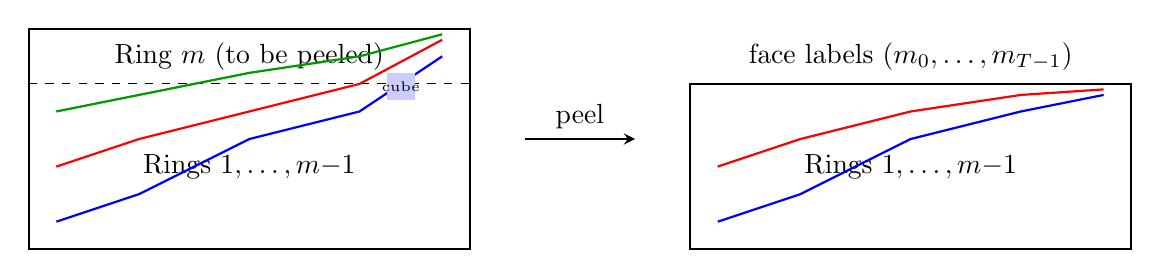
\begin{tikzpicture}[scale=0.7, >=stealth]
  % Tower
  \draw[thick] (0,0) rectangle (8,4);
  \draw[dashed] (0,3) -- (8,3);
  \node at (4, 3.5) {Ring $m$ (to be peeled)};
  \node at (4, 1.5) {Rings $1, \ldots, m{-}1$};

  % Paths (schematic)
  \draw[thick, blue] (0.5, 0.5) -- (2, 1) -- (4, 2) -- (6, 2.5)
    -- (7.5, 3.5);
  \draw[thick, red] (0.5, 1.5) -- (2, 2) -- (4, 2.5) -- (6, 3)
    -- (7.5, 3.8);
  \draw[thick, green!60!black] (0.5, 2.5) -- (2, 2.8) -- (4, 3.2)
    -- (6, 3.5) -- (7.5, 3.9);

  % Cubes
  \fill[blue!20] (6.5, 2.7) rectangle (7, 3.2);
  \node at (6.75, 2.95) {\tiny cube};

  % Arrow
  \draw[->, thick] (9, 2) -- (11, 2) node[midway, above] {peel};

  % After peel
  \draw[thick] (12, 0) rectangle (20, 3);
  \node at (16, 1.5) {Rings $1, \ldots, m{-}1$};
  \node at (16, 3.5) {face labels $(m_0, \ldots, m_{T-1})$};
  \draw[thick, blue] (12.5, 0.5) -- (14, 1) -- (16, 2) -- (18, 2.5)
    -- (19.5, 2.8);
  \draw[thick, red] (12.5, 1.5) -- (14, 2) -- (16, 2.5) -- (18, 2.8)
    -- (19.5, 2.9);
\end{tikzpicture}
\end{center}


\subsection{Gluing a ring = adding a new top level}

Gluing reverses the peel: given the $m{-}1$ level tower and face
labels $(m_0, \ldots, m_{T-1})$, the forward Burge rule reconstructs
the top-level paths.  The face labels determine where the new
top-level paths go: each cube (face label unit) inserts a new
path-step, extending the paths upward.

In terms of the involution on triples $(S, U, \nu)$, the two
fundamental moves (Definition~\ref{def:two-moves}) have transparent
NILP interpretations:

\begin{itemize}
  \item \textbf{Move~S (peel direction):}
    Remove the top level of the NILP tower: collapse the three paths
    at level~$m$ into the crossing marker $m \in S$.  The extracted
    face labels encode the path geometry at the removed level.
    The tower shrinks: $m \to m-1$.

    \smallskip
    \textbf{Move~S (glue direction):}
    Restore a level: take $k \in S$, reconstruct face labels from the
    weight budget, and apply the forward rule to build new top-level
    paths.  The tower grows: $m \to m+1$.

  \item \textbf{Move~U (peel direction):}
    The tower keeps the same height~$m$.  Instead, modify the face
    labels at ring~$i$ \emph{within} the tower, extracting $i$~units
    of weight and storing them as the Euler mark $i \in U$.
    In NILP terms: remove $i$~cubes from the interior of the path
    family (tighten the gaps between paths at specific steps).

    \smallskip
    \textbf{Move~U (glue direction):}
    Take the mark $i \in U$ and inject $i$~cubes back into the
    interior (widen the gaps between paths at specific steps).
\end{itemize}

\noindent
Every involution step---without exception---is either a peel
(extracting structure from the tower into~$S$ or~$U$) or a glue
(injecting structure from~$S$ or~$U$ back into the tower).  The
canonical choice of which to perform at each non-fixed-point triple
is the open problem (Section~\ref{sec:canonical}).


\subsection{Compression = a partially disassembled tower}
\label{sec:nilp-compression}

The two operations combine to give a NILP picture of
compression (Definition~\ref{def:compression}).
A triple $(S, U, \nu)$ with $m = n - |S|$ represents a tower
that has been \textbf{partially disassembled} in two ways:

\begin{enumerate}
  \item \textbf{Floors removed} (structural compression, $S$).
    Each $k \in S$ records a level that has been crushed out of
    the tower.  The three paths at that level are gone; the
    levels above have collapsed down.  The tower shrinks from
    $n$~levels to $m$~levels.

    \smallskip
    Concretely: in a tower of height~$n = 3$ with
    $S = \{2\}$, the second floor is removed and the third
    floor becomes the new second.  The cubes that filled the
    gap between levels~$1$ and~$2$ are extracted as face labels,
    then discarded (their total weight~$b_2$ is absorbed into
    $\sigma(S)$).

  \item \textbf{Floors thinned} (weight compression, $U$).
    Each $i \in U$ records a level where cubes have been
    extracted from the interior.  The paths at level~$i$ remain,
    but the gap between levels~$i{-}1$ and~$i$ has been
    tightened: exactly $i$~cubes are missing compared to the
    uncompressed tower.

    \smallskip
    Concretely: if $U = \{2\}$ in a tower of height~$m = 3$,
    then $2$~cubes have been removed from ring~$2$---the paths
    at levels~$1$ and~$2$ are closer together at two of the
    $T$~steps around the cylinder.
\end{enumerate}

\noindent
The residual CPP~$\nu$ is whatever remains: a valid NILP tower
of height~$m$, with thinner gaps at the marked rings.

\begin{center}
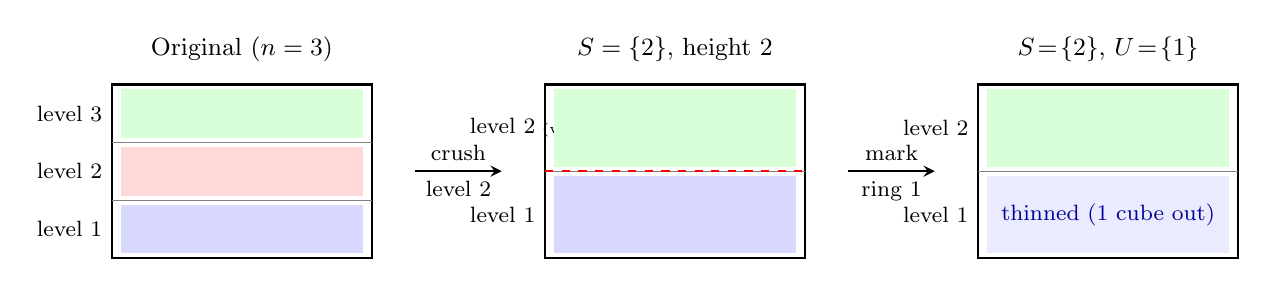
\begin{tikzpicture}[scale=0.55, >=stealth]
  % Original tower
  \node[above] at (3, 4.3) {\small Original ($n = 3$)};
  \draw[thick] (0,0) rectangle (6,4);
  \draw[thin, gray] (0,1.33) -- (6,1.33);
  \draw[thin, gray] (0,2.66) -- (6,2.66);
  \node[left, font=\footnotesize] at (0, 0.66) {level 1};
  \node[left, font=\footnotesize] at (0, 2.0) {level 2};
  \node[left, font=\footnotesize] at (0, 3.33) {level 3};
  % Cubes (schematic fills)
  \fill[blue!15] (0.2,0.1) rectangle (5.8,1.23);
  \fill[red!15] (0.2,1.43) rectangle (5.8,2.56);
  \fill[green!15] (0.2,2.76) rectangle (5.8,3.9);

  % Arrow 1
  \draw[->, thick] (7, 2) -- (9, 2)
    node[midway, above, font=\footnotesize] {crush}
    node[midway, below, font=\footnotesize] {level 2};

  % After S = {2}
  \node[above] at (13, 4.3) {\small $S = \{2\}$, height $2$};
  \draw[thick] (10,0) rectangle (16,4);
  \draw[thin, gray] (10,2) -- (16,2);
  \node[left, font=\footnotesize] at (10, 1.0) {level 1};
  \node[left, font=\footnotesize] at (10, 3.0) {level 2\rlap{\;\tiny(was 3)}};
  \fill[blue!15] (10.2,0.1) rectangle (15.8,1.9);
  \fill[green!15] (10.2,2.1) rectangle (15.8,3.9);
  % Removed floor
  \draw[dashed, red, thick] (10, 2) -- (16, 2);

  % Arrow 2
  \draw[->, thick] (17, 2) -- (19, 2)
    node[midway, above, font=\footnotesize] {mark}
    node[midway, below, font=\footnotesize] {ring 1};

  % After U = {1}
  \node[above] at (23, 4.3)
    {\small $S\!=\!\{2\}$, $U\!=\!\{1\}$};
  \draw[thick] (20,0) rectangle (26,4);
  \draw[thin, gray] (20,2) -- (26,2);
  \node[left, font=\footnotesize] at (20, 1.0) {level 1};
  \node[left, font=\footnotesize] at (20, 3.0) {level 2};
  \fill[blue!8] (20.2,0.1) rectangle (25.8,1.9);
  \fill[green!15] (20.2,2.1) rectangle (25.8,3.9);
  % Indicate thinned gap
  \node[font=\footnotesize, blue!60!black] at (23, 1.0)
    {thinned ($1$ cube out)};
\end{tikzpicture}
\end{center}

\noindent
The two compressions differ in their effect on the tower:
\begin{center}
\renewcommand{\arraystretch}{1.3}
\begin{tabular}{l|l|l}
  & \textbf{Structural ($S$)}
  & \textbf{Weight ($U$)} \\ \hline
  Tower height & decreases by $1$
  & unchanged \\
  Paths at that level & removed entirely
  & remain, gaps tightened \\
  Cubes affected & all cubes at one level
  & exactly $i$ cubes thinned \\
  Reversal & glue: needs face labels
  & glue: re-insert $i$ cubes
\end{tabular}
\end{center}

\noindent
To \textbf{reconstruct} the original $n$-level tower from
$(S, U, \nu)$: first undo the $U$-marks (inject cubes back into
the thinned rings), then undo the $S$-crushes (glue the removed
floors back, from bottom to top).


%% ============================================================
\section{The $n = 1$ case: injection as cube addition}
\label{sec:n1}
%% ============================================================

For $n = 1$, the ground set simplifies dramatically.  There are only
three types of triples:

\begin{center}
\renewcommand{\arraystretch}{1.3}
\begin{tabular}{l|c|c|l}
\textbf{Triple} & \textbf{Sign} & \textbf{Weight} &
  \textbf{Meaning}
\\ \hline
$(\emptyset, \emptyset, \nu)$, $\max(\nu) = 1$
  & $+1$ & $|\nu|$
  & unmarked NILP family
\\
$(\emptyset, \{1\}, \nu)$, $\max(\nu) = 1$
  & $-1$ & $1 + |\nu|$
  & Euler-marked NILP family
\\
$(\{1\}, \emptyset, \nu_\emptyset)$, $\max(\nu_\emptyset) = 0$
  & $-1$ & $1$
  & crossed (empty CPP)
\end{tabular}
\end{center}

The involution must pair each negative triple with a distinct positive
triple of the same weight.  At weight~$w$:
\begin{itemize}
  \item Positive triples: CPPs with $\max = 1$ and weight $w$.
    Count: $f_1(w) := [q^w]\,f_{1,c}(q)$.
  \item Negative triples:
    \begin{itemize}
      \item Euler-marked CPPs with weight $w - 1$.
        Count: $f_1(w-1)$.
      \item One crossed triple (only at $w = 1$).
    \end{itemize}
\end{itemize}

For $w \geq 2$, the involution reduces to an \textbf{injection}:
\begin{equation}\label{eq:injection}
  \varphi\colon \{\text{CPPs with } \max = 1,\, |\nu| = w-1\}
  \;\hookrightarrow\;
  \{\text{CPPs with } \max = 1,\, |\nu| = w\}.
\end{equation}
The image of~$\varphi$ pairs with the Euler-marked triples; the
non-images are the fixed points of the involution, contributing
to~$Q_{1,c}(q)$.

In NILP terms, $\varphi$ adds one cube to the NILP family:
\[
  \varphi(\nu) = \nu + \text{one cube at a canonical position}.
\]
Each CPP $\nu = (\nu^1, \nu^2, \nu^3)$ with $\max = 1$ has
partitions $\nu^i = (1^{a_i})$.  Adding a cube means appending
a row to one of the three partitions: $a_k \to a_k + 1$ for some
$k \in \{1, 2, 3\}$.

The \textbf{slack vector} $s = (s_1, s_2, s_3)$, where
$s_k = a_k - a_{k-1 \bmod 3} + c_{k-1 \bmod 3}$ measures the room
available for each path, determines which paths can be extended:
path~$k$ can receive a cube if and only if $s_k > 0$.


%% ============================================================
\section{The $d \equiv 0 \pmod{3}$ obstruction}
\label{sec:d0}
%% ============================================================

For $d \equiv 0 \pmod{3}$, the CPP weight distribution at $\max = 1$
oscillates with period~$3$:
\[
  f_1(w) =
  \begin{cases}
    d/3 + 1 & \text{if } w \equiv 0 \pmod{3}, \\
    d/3     & \text{otherwise}.
  \end{cases}
  \qquad\text{(for $w$ sufficiently large).}
\]
The extra CPP at weights $w \equiv 0 \pmod{3}$ is the
\emph{balanced} configuration $\nu = (1^{a}, 1^{a}, 1^{a})$ with
slack $(a, a, a)$ (equal room in all three directions).

The injection~\eqref{eq:injection} maps CPPs of weight~$w$ into CPPs
of weight~$w+1$.  At weights $w \equiv 0 \pmod{3}$ (where there are
$d/3 + 1$ CPPs) mapping to $w+1 \equiv 1 \pmod{3}$ (where there are
only $d/3$ CPPs), the injection has a \textbf{deficit}: more sources
than targets.

This deficit is exactly why $Q_{1,c}(q)$ has negative coefficients
when computed with $(q)_1 = 1 - q$.  The conjecture resolves this by
using $(q^\ell; q^\ell)_n$ with $\ell = \gcd(d, 3) = 3$: the factor
$(1 - q^3)$ has the correct periodicity to match the period-$3$
oscillation, absorbing the deficit.


%% ============================================================
\section{Summary}
\label{sec:summary}
%% ============================================================

\begin{center}
\renewcommand{\arraystretch}{1.4}
\begin{tabular}{l|l|l}
\textbf{Operation} & \textbf{Growth diagram} & \textbf{NILP tower}
\\ \hline
Peel (inverse rule)
  & Remove outermost ring;
  & Remove top level of tower; \\
  & extract face labels
  & extract cubes as face labels
\\ \hline
Glue (forward rule)
  & Add outermost ring;
  & Add top level to tower; \\
  & insert face labels
  & insert cubes from face labels
\\ \hline
Move~S (crossing)
  & Peel/glue ring~$m$;
  & Collapse/expand top-level \\
  & trade level $\leftrightarrow$ $S$
  & paths $\leftrightarrow$ crossing marker
\\ \hline
Move~U (Euler mark)
  & Redistribute weight at
  & Tighten/widen gaps at ring~$i$; \\
  & ring~$i$; trade weight $\leftrightarrow$ $U$
  & trade cubes $\leftrightarrow$ Euler mark
\end{tabular}
\end{center}

\noindent
Move~C (cross-to-mark conversion) is sign-neutral and does
not appear as a standalone involution step
(Remark~\ref{rmk:two-not-three}).


\begin{thebibliography}{99}
\bibitem{UNDERLYING_SET}
  R.~Langer,
  \emph{The Underlying Set: Cylindric Plane Partitions, ALCDs,
  and the Ground Set for the Involution},
  companion note, 2026.

\bibitem{Q_NILP}
  R.~Langer,
  \emph{$Q$-Non-Intersecting Lattice Paths},
  companion note, 2026.

\bibitem{INVOLUTION}
  R.~Langer,
  \emph{The Recursive Franklin Involution for Cylindric
  Partition Positivity},
  companion note, 2026.

\bibitem{langer-thesis}
  R.~Langer,
  \emph{Cylindric Partitions and Bijective Proofs},
  PhD thesis, University of Melbourne.
\end{thebibliography}

\end{document}
